\section{Serverless Architecture}\label{sec:architecture}

We used a Serverless Architecture to deploy all the work.

To offer the application to end-users with high availability and high performance we deployed all Javascript files that are part of the system into a CDN (Content Delivery Network). This single point of deploy offered us a centralized method to upgrade all customers applications, whereby there is a new version, without any customer explicit action.

To perform CPU intensive operations, necessary to make complex geometric element, we used a third party FaaS system that run Python functions and that generate 3D elements. Thank to this we can scale up and down and adjust the CPU load on the traffic.

The application is distributed as frontend web application and so it's mostly executed into customer's browser. This has the following advantages: (i) to avoid user hard installation or updating typically performed by not technical users; (ii) to offer a good abstraction level that makes the application platform and operation system independent;  (iii) to avoid a server overloading by moving heavy computations on the user client.

The application state is mostly inside the customer's browser and it is represented as a tree structured object. This state can be serialized and saved on a BaaS system or downloaded as JSON file. The customer can restore the application state in any time using a preceding downloaded serialized version of the state. The system will adjust the user interface and the scene by means of the Virtual DOM and the diff and patch algorithm.

The collaboration part is based on a DBaaS, with the common state stored in an external DB provided by Firebase. Following this methodology we could also add user authentication features based on external BaaS providing all user management functionalities.

In Figure~\ref{fig_serverless} there is the architectural schema described above\\\\

\begin{figure}[htb]
\centering
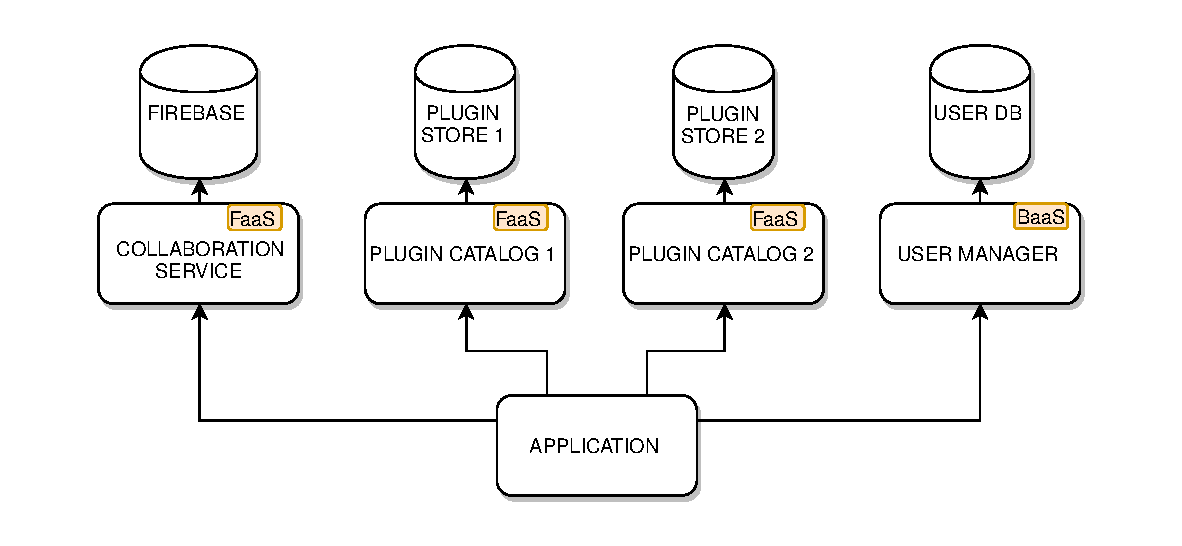
\includegraphics[width=\linewidth]{contents/images/serverless-diagram}

\caption{The serverless architecture for our application.}
\label{fig_serverless}
\end{figure}



\subsection{Centralized Application State}\label{ssub:centr_state}

blabla

\subsection{Component Based UI}


blabla